\documentclass[titlepage]{report}

\usepackage[toc,page]{appendix}
\usepackage{glossaries}
\usepackage{makeidx}
\usepackage{biblatex}
\usepackage{graphicx}
\usepackage{float}

\makeglossaries{}
\loadglsentries{entries}

\makeindex
\addbibresource{bib.bib}

\title{blockchain\_message: A Peer-to-Peer Content-Sharing Service Built on the Ethereum Blockchain\\\large System Design}
\author{Sean T. Batzel\\Dr.\ Bishop}
\date{\today\endgraf\bigskip Submitted in partial fulfillment of the requirements of CMPS/IT 490 --- Computer Projects}

\begin{document}
\maketitle

\tableofcontents

\nocite{*}

\begin{abstract}
    Formally, blockchain\_message is the combination of the specification of a library interface which provides the ability to securely send immutable messages through \gls{Ethereum}\index{Ethereum} and a set of smart contracts running on the EVM\index{EVM} that implement remote communication. The end goal for the senior project is to have a CLI\index{CLI} client which is able to implement every function outlined in the description of the system's design. Eventually, my hope is to also have blockchain\index{blockchain}\_message implemented as an Android application and a graphical desktop application.
\end{abstract}

\section{System Architectural Design}
The system's architecture is mostly based in the abstract standard for the client library (discussed in the \textbf{Component Architectural Design} section) and a set of \glspl{smart contract}\index{smart contracts} which create the actual body of the system.

\subsection{Accomplished Functionality}
\subsubsection{Communication Implementation}
Messages are handled by a simple \gls{smart contract}\index{smart contract} which is capable of storing and retrieving messages from \gls{Ethereum}\index{Ethereum} permanent storage. Internally, this is accomplished with a two-dimensional array. When a message $x$ is sent, it is assigned to the array with the indices $x[user\_id][msg\_id]$.

\begin{figure}[tph!]
    \centering
    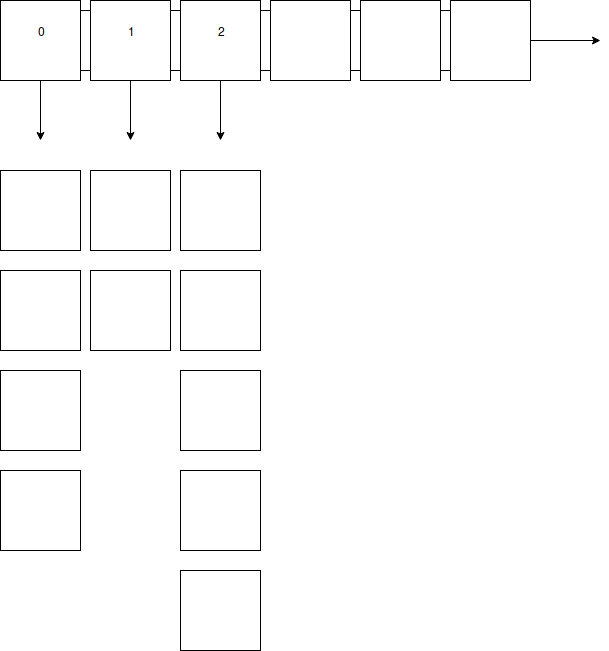
\includegraphics[width=0.7\linewidth]{message_storage}
    \caption{A graphical representation of the BlckchnMsgStorage internal array. The array contains three initialized contacts with a variable number of messages each.}
    \label{fig:messagestorage}
\end{figure}

\subsubsection{Identity Management}
\gls{Identity management} is one of the high-level stretch goals outlined in the original proposal, and will need a new \gls{smart contract}\index{smart contract} written which will be capable of attaching a single unique user id (\texttt{addr}) with a single username/email/password set, thereby preventing messages from being sent to the wrong person, similar to a phone number. The \texttt{BlckchnMsgStorage} contract itself only deals with the user's address\index{address}, and without some kind of user management and address\index{address} assignment to act as a key any person would be able to tie in to any address\index{address} and download every message in that address\index{address}'s associated ``mailbox''. The smart contract will contain a key-value lookup table where every new login is assigned an address\index{address} which is immutably tied to that username. When adding a contact, the only values supplied will be a username and email address\index{address}, which the identity management contract will use to retrieve an address\index{address} which is never exposed to the end user.

\subsection{Functionality Goals}
\subsubsection{Key Management}
Key management is usually handled through well-known servers set up specifically for distributing public keys. Because the keys used with this system are not OpenPGP-standardized, this method may not work as cleanly. Further work will be done to determine the remote key management system that makes the most sense for this platform. Internally to a client application, keys are read from files and are then stored in memory as binary public key\index{public key} objects. Each implementation will require its own language's approach to this, for example the Android app will use net.java.Security.PublicKey\index{PublicKey} and the Python implementation (CLI\index{CLI}) will use rsa.PublicKey\index{PublicKey}, both from their language's standard library. Keys, in the initial release of the application, must be exported (either by manually copying the keyfile from the keys directory or by using the eventual Export functionality)\footnote{At the time of writing, the ``Import'' and ``Export'' functionality groups are not yet implemented. When every basic feature of the applications is in place and working, abstraction functions like these will be added.} and sent (by email or similar medium) to the intended contact, who will then move it into their own keys directory (either manually or by using the eventual Import functionality) to be imported when the new Contact object is created.

\section{Component Architectural Design}

\subsection{Blockchain Communication}
The Blockchain module is used to send and retrieve message packets serialized as strings.

\subsubsection{def get\_identity(self, uname: str) $\rightarrow$ int}
Either produces a new address by which a new user can be contacted or retrieves an existing user's unique address.
\subsubsection{def get\_my\_identity(self, uname: str, password: str) $\rightarrow$ int}
\subsubsection{def new\_identity(self, uname: str, password: str) $\rightarrow$ int}
\subsubsection{def get\_balance(self) $\rightarrow$ float}
Returns the volume of \gls{Ether}\index{Ether} (ETH) the user has in their account. This is used to ensure that a user can always keep track of their ETH\index{ETH} and to keep from running out of currency to cover the gas fees associated with sending messages.
\subsubsection{def submit(self, message: Message)}
Produces a message packet from a database Message object and transmits it to the \gls{blockchain}\index{blockchain}.
\subsubsection{def retrieve(user: Contact, last\_message: int, contact\_list: List[Contact]) $\rightarrow$ List[Message]}
Requests every message packet with an ID later than \texttt{last\_message}, receives a string containing each message packet, and processes the string to pass of for cryptographical processing.

\subsection{Low-Level Cryptography}
This module will provide an abstraction level to an internal language-level implementation of RSA\index{RSA} public/private key encryption\index{encryption}.

\subsubsection{def generate\_key(uname: str)}
Used when logging in for the first time on a new device. Produces a new RSA\index{RSA} keypair.
\subsubsection{def import\_key(uname: str)}
Brings an existing RSA\index{RSA} keypair into memory for application use.
\subsubsection{def encrypt(to: Contact, msg: str) $\rightarrow$ str}
Encrypts a given string \texttt{msg} for decryption by \texttt{to}.
\subsubsection{def decrypt(msg: str) $\rightarrow$ str}
Decrypts messages encrypted with the currently signed-in user's encryption\index{encryption} key.
\subsubsection{def sign(msg: Message) $\rightarrow$ str}
Produces a text-encoded signature\index{signature} for the given message which can then be used to verify the identity of the sender.
\subsubsection{def verify(from: Contact, msg: Message) $\rightarrow$ bool}
Verifies that a message originates with the sender it claims to be from.

\subsection{Database Design}
The database specification is to provide a language-native ``list'' implementation of each necessary object for comparably efficient and low-level data storage and retrieval. These will be frozen in place and saved to files (by way of libraries and utilities like Python's \texttt{shelve}) that will be read and written in chunks which will remove the need for large, complex database files with a more prohibitive overhead. The specific data structures and their interactions are outlined in the \textbf{Data Structure Overview}. Each operation that updates the state of the in-memory database (insert/delete) will cause the database to update on disk as well.

\subsubsection{def insert(msg: Message) $\rightarrow$ bool}
Creates a new database entry with the given Message object.
\subsubsection{def read(id: int) $\rightarrow$ Message}
Returns the message with the given unique identifier.
\subsubsection{def delete(id: int) $\rightarrow$ bool}
Removes the message with the given unique identifier. DOES NOT modify the message records on the \gls{blockchain}\index{blockchain}.
\subsubsection{def new\_contact(addr: int, uname: str, email: str) $\rightarrow$ bool}
Produces a new contact from the given information and adds it to the in-memory database.
\subsubsection{def read\_contact(self, uname: str) $\rightarrow$ Contact}
\subsubsection{def del\_contact(addr: int) $\rightarrow$ bool}
Removes a given contact (identified by \texttt{addr} from the database.)

\section{Real-Time Design}
Real-time interactions are limited by the responsivity and reactivity of \gls{Ethereum}\index{Ethereum}. For multiple users sharing a local node\index{node}, the transmission of messages across blockchains\_message is instantaneous. For a number of node\index{node}s connecting together the transmission of messages is limited by a myriad of factors including the user's network speed and the number of transactions\index{transactions} being processed by \gls{Ethereum}\index{Ethereum} as a whole. When a message is sent, a new transaction\index{transaction} is appended to the \gls{blockchain}\index{blockchain} containing the information relevant to the message being sent. This must propagate through \gls{Ethereum}\index{Ethereum} before it can be loaded into blockchain\_message by the intended recipient, which introduces a delay which is noticeable but not strictly prohibitive.

\section{User Interface Design}
Any implementation of the system should provide a clear, usser-friendly manner of exposing every function of the library to the user. It should also focus heavily on abstracting complex tasks such as key management\index{key management} from the user and presenting such intensive actions in as clear and simple a manner as possible. For the purposes of this project, two implementations are currently under development, the command-line interface that encompasses the end goal of the UI component of the project, and an Android application that will explore the practicality of using a mobile device for such a task.

\subsection{Command-Line Interface}
The CLI\index{CLI} implementation provides all of the basic functions of the system in a bare-bones, low abstraction manner. Each high-level operation provided by the blockchain\_message system should have a 1:1 relationship with a single command (e.g. write message, download messages, read messages, list contacts, et cetera).

\subsection{Graphical/Mobile}
Graphical implementations of blockchain\_message, including the Android application being developed for this project, should provide a highly user-friendly and abstracted way of interacting with the underlying platform.

\section{Help System Design}

\subsection{CLI\index{CLI}}
The CLI\index{CLI} version will include a standard \verb|help| directive that will print out the full list of commands available with usage details for every component in the style of classical *nix command help dialogues. The user manual will also contain specific information on the usage of the CLI version, since that will most directly reflect the functionality described in the original proposal.

\subsection{Graphical/Mobile}
The graphical implementations (starting with the Android app) will contain a help dialog, clearly labeled as part of an auxiliary menu, that will display a clear overview of how every component of the UI will function as well as basic overviews of cryptographical functions and how to interact with an individual \gls{Ethereum}\index{Ethereum} account.

\section{Data Structure Overview}
\subsection{Contact}
Every person that the user interacts with will be stored as a Contact object such that the system can easily exchange messages while maintaining a high level of convenience for the end user.

\subsubsection{addr}
A numerical identifier providing the system with a simple way of addressing and indexing messages.

\subsubsection{uname}
The contact's chosen username, which will be used internally to connect an \texttt{addr} with a more intuitive name and ensure that each address\index{address} is only used once per blockchain\_message environment.

\subsubsection{emailAddress}
The user's given email address\index{address}, which will be used to identify public encryption\index{encryption} keys.

\subsubsection{publicKey}
The public key\index{public key} associated with the given email address\index{address}, stored as Java's internal PublicKey\index{PublicKey} class, Python's rsa.PublicKey\index{PublicKey} class, or a similar data structure.

\subsection{Message}
This data object will be 

\subsubsection{id}
A unique identifier supplied to each message.

\subsubsection{to}
The unique user address\index{address} for the person receiving the message.

\subsubsection{from}
The unique user address\index{address} for the person sending the message.

\subsubsection{text}
Used to store the plaintext \textit{and} ciphertext representations of the message being sent.

\subsubsection{sign}
Contains a text-encoded representation of the RSA\index{RSA} signature\index{signature} applied to the plaintext message.

\subsubsection{verified}
A Boolean value used in client implementations to easily store whether or not the message has been cryptographically verified. When sending to \gls{Ethereum}\index{Ethereum} this will default to false.

\pagebreak

\section{Progress to Date}

\begin{table}[ht]
\begin{center}
\caption{Progress on Individual Project Elements}
\begin{tabular}{| l | p{5cm} |}
\hline
Proposed Project Specifications & \textbf{Complete} \\
\hline
Command-line Interface & \textbf{Complete} \\
Local Database Implementation & \textbf{Complete} \\
RSA\index{RSA} Encryption/Decryption & \textbf{Complete} \\
RSA\index{RSA} Signing and Verification & \textbf{Complete} \\
Smart Contract Message Handling & \textbf{Complete} \\
\hline
Identity and Cryptography Stretch Goals & \textbf{To Be Completed by November First} \\
\hline
Smart Contract Identity Assignment & \textbf{Complete} \\
Public-key Sharing & \textbf{Currently manual} \\
Key Signing & \textbf{Not Started} \\
\hline
Client Implementation Stretch Goals & \textbf{Concept Goal} \\
\hline
Server Implementation & \textbf{Not Started} \\
HTML5 Interface & \textbf{Not Started} \\
Android Application & \textbf{In Progress} \\
\hline
\end{tabular}
\end{center}
\end{table}

\listoftables
\listoffigures
\printindex
\printglossaries{}
\printbibliography{}

\end{document}
